\documentclass[11pt,compress,t,notes=noshow, aspectratio=169, xcolor=table]{beamer}

\usepackage{../../style/lmu-lecture}
% Defines macros and environments
% This file is included in slides and exercises

% Rarely used fontstyle for R packages, used only in 
% - forests/slides-forests-benchmark.tex
% - exercises/single-exercises/methods_l_1.Rnw
% - slides/cart/attic/slides_extra_trees.Rnw
\newcommand{\pkg}[1]{{\fontseries{b}\selectfont #1}}

% Spacing helpers, used often (mostly in exercises for \dlz)
\newcommand{\lz}{\vspace{0.5cm}} % vertical space (used often in slides)
\newcommand{\dlz}{\vspace{1cm}}  % double vertical space (used often in exercises, never in slides)
\newcommand{\oneliner}[1] % Oneliner for important statements, used e.g. in iml, algods
{\begin{block}{}\begin{center}\begin{Large}#1\end{Large}\end{center}\end{block}}

% Don't know if this is used or needed, remove?
% textcolor that works in mathmode
% https://tex.stackexchange.com/a/261480
% Used e.g. in forests/slides-forests-bagging.tex
% [...] \textcolor{blue}{\tfrac{1}{M}\sum^M_{m} [...]
% \makeatletter
% \renewcommand*{\@textcolor}[3]{%
%   \protect\leavevmode
%   \begingroup
%     \color#1{#2}#3%
%   \endgroup
% }
% \makeatother


\tikzset{main node/.style={rectangle,draw,minimum size=1cm,inner sep=4pt},}

\title{Interpretable Machine Learning}
% \author{LMU}
%\institute{\href{https://compstat-lmu.github.io/lectureml/}{compstat-lmu.github.io/lecture\ml}}
\date{}

\def\firstrowcolor{}
\def\secondrowcolor{}
\def\thirdrowcolor{}
\def\fourthrowcolor{}

\usepackage{tikz}

\begin{document}

\newcommand{\titlefigure}{figure/ebm.jpg}
\newcommand{\learninggoals}{
% \item Model-based boosting with simple base learners
% \item Feature effect and importance in model-based boosting}
\item Motivation from GAM
\item Intelligible GAM
\item Accurate GAM + Pairwise Interactions
\item FAST feature interaction detection}

\lecturechapter{Explainable Boosting Machines}
\lecture{Interpretable Machine Learning}

\begin{frame}{Explainable Boosting Machines (EBM) \citebutton{Lou et al. 2012}{https://www.cs.cornell.edu/~yinlou/papers/lou-kdd12.pdf}}
\textbf{Recall GAM}: 
$$
g\big(\mathbb{E}[y \mid \mathbf{x}]\big) = \theta_0 + f_1(x_{1}) + f_2(x_{2}) + \ldots + f_p(x_{p}),
$$

\begin{itemize}
    \item One shape function $f_j$ per feature $x_j$\\ $\leadsto$ \textbf{Feature-level interpretability}
    \item Captures non-linear univariate effects\\ $\leadsto$ \textbf{Better performance / more flexible than GLMs}
\end{itemize}

\medskip

\textbf{Idea of EBM:} \textbf{GAMs} trained with \textbf{gradient boosting} over \textbf{shallow bagged trees}
\begin{itemize}
    \item \textbf{GAMs} - provide feature-wise interpretability via separate shape functions $f_j(x_j)$\\
    $\leadsto$ Potentially include pairwise interactions
    \item \textbf{Gradient Boosting} - incrementally fits residuals to improve predictive performance while retaining additivity
    \item \textbf{Shallow Bagged Trees} - low-depth trees (2–4 leaves) reduce variance and create interpretable shape functions
\end{itemize}

% \textbf{Idea of EBM}: \textbf{GAMs} trained with \textbf{gradient boosting} over \textbf{shallow bagged trees}\\

%     \begin{itemize}
%         \item Interpretable like GAMs
%         \item Accuracy close to unrestricted ensembles (e.g., random forests)
%     \end{itemize}

\end{frame}




\begin{frame}{EBM - Two-Stage Model Construction}
\begin{enumerate}
    \item \textbf{Stage 1: Fit Main Effects (Univariate Terms)}
    \begin{itemize}
        \item Train EBM using only feature-wise shape functions $f_j(x_j)$
        \item Freeze the univariate model after convergence
    \end{itemize}
    
    \item \textbf{Stage 2: Add Selected Pairwise Interactions}
    \begin{itemize}
        \item Apply \textbf{FAST} to rank all $O(p^2)$ feature pairs by potential reduction in RSS
        \item User or heuristic selects top $K$ interactions and stores them in $\mathcal{K}$
        \item Use boosting to fit pairwise terms $f_{ij}(x_i, x_j)$ on residuals
        \item Final model: $\hat{f}(\xv) = \sum_{j=1}^p f_j(x_j) + \sum_{(i,j)\in\mathcal{K}} f_{ij}(x_i, x_j)$
    \end{itemize}
\end{enumerate}

% 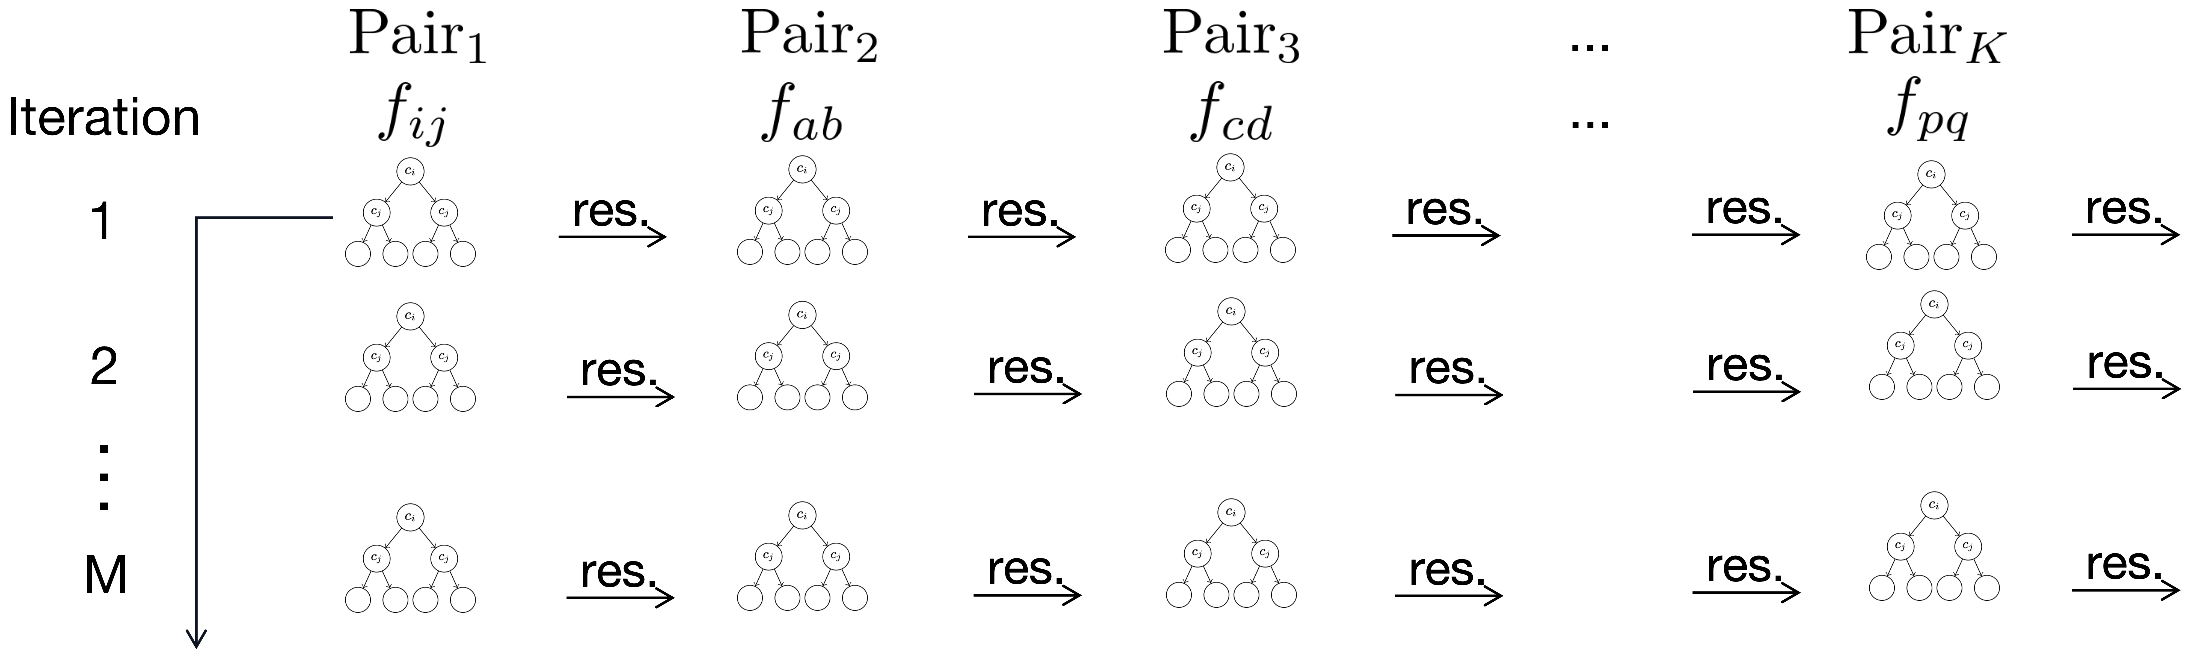
\includegraphics[width=1\linewidth]{figure/GA2M_Step1.png}
\end{frame}



\begin{frame}{EBM Stage I - Initialization}

%\textbf{Initialization:}
\begin{itemize}
    \item Set all shape functions to zero:
    $$
    f_j^{(0)}(x_j) = 0 \quad \text{for all } j = 1, \dots, p
    $$
    \item Compute initial model prediction:
    $$
    \hat{y}^{(0)} = \sum_{j=1}^p f_j^{(0)}(x_j) = 0
    $$
    \item Compute initial pseudo-residuals (e.g., for squared loss):
    $$
    \tilde{r}^{(0)} = -\frac{\partial L}{\partial \hat{y}} = y - \hat{y}^{(0)} = y
    $$
\end{itemize}

\end{frame}

\begin{frame}{EBM Stage I – First Feature Update}
\begin{figure}
    \centering
    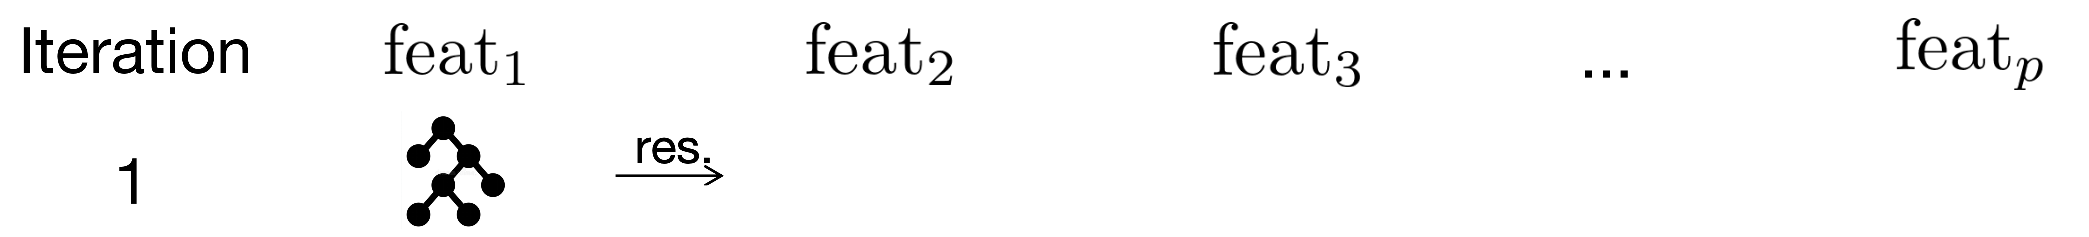
\includegraphics[width=\linewidth]{figure/EBM_Step1.png}
\end{figure}
\begin{itemize}
    \item Fit shallow bagged tree $S_1^{(1)}$ (2–4 leaves) to training data $\left\{\left(x_1, \tilde{r}^{(0)}\right)^{(i)}\right\}_{i=1}^n$\\
    $\leadsto$ Use only feature $x_1$ as input and $\tilde{r}^{(0)}$ as target
    \item Update first shape function:
    $$
    f_1^{(1)}(x_1) = f_1^{(0)}(x_1) + \eta \cdot S_1^{(1)}(x_1)
    $$
    \item Update prediction:
    $$
    \hat{y}^{(1)} = \sum_{j=1}^p f_j^{(1)}(x_j)
    $$
    \item Recompute pseudo residuals:
    $$
    \tilde{r}^{(1)} = y - \hat{y}^{(1)}
    $$
\end{itemize}

\end{frame}


\begin{frame}{EBM Stage I – Cycle Through Features}
\begin{figure}
    \centering
    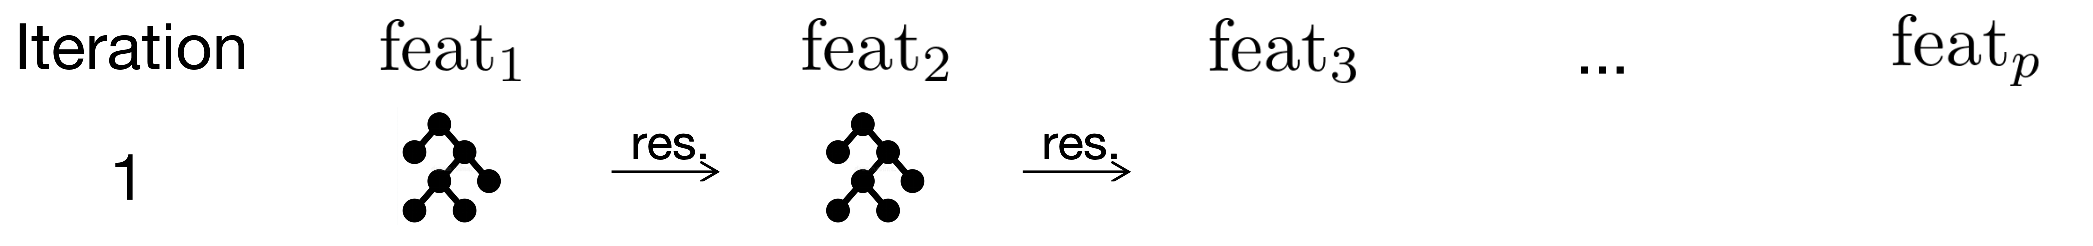
\includegraphics[width=\linewidth]{figure/EBM_Step2.png}
\end{figure}
\begin{itemize}
    \item 1st boosting iteration: \\
    Cycle through each feature $j = 2,\dots,p$:
    \begin{itemize}
        \item Fit shallow bagged tree $S_j^{(1)}$ using feature $x_j$ and previous residual $\tilde{r}^{(j-1)}$ %to $(x_j, \tilde{r}^{(j-1)})$
        \item Update $f_j$: $f_j^{(1)}(x_j) = f_j^{(0)}(x_j) + \eta \cdot S_j^{(1)}(x_j)$
        \item Recompute $\hat{y}$ and residuals: $\tilde{r}^{(j)} = y - \hat{y}^{(j)}$
    \end{itemize}
    \item After one full pass over features, we complete one boosting iteration
\end{itemize}
\end{frame}

\begin{frame}{EBM Stage I – Iterate Boosting Process}
\begin{figure}
    \centering
    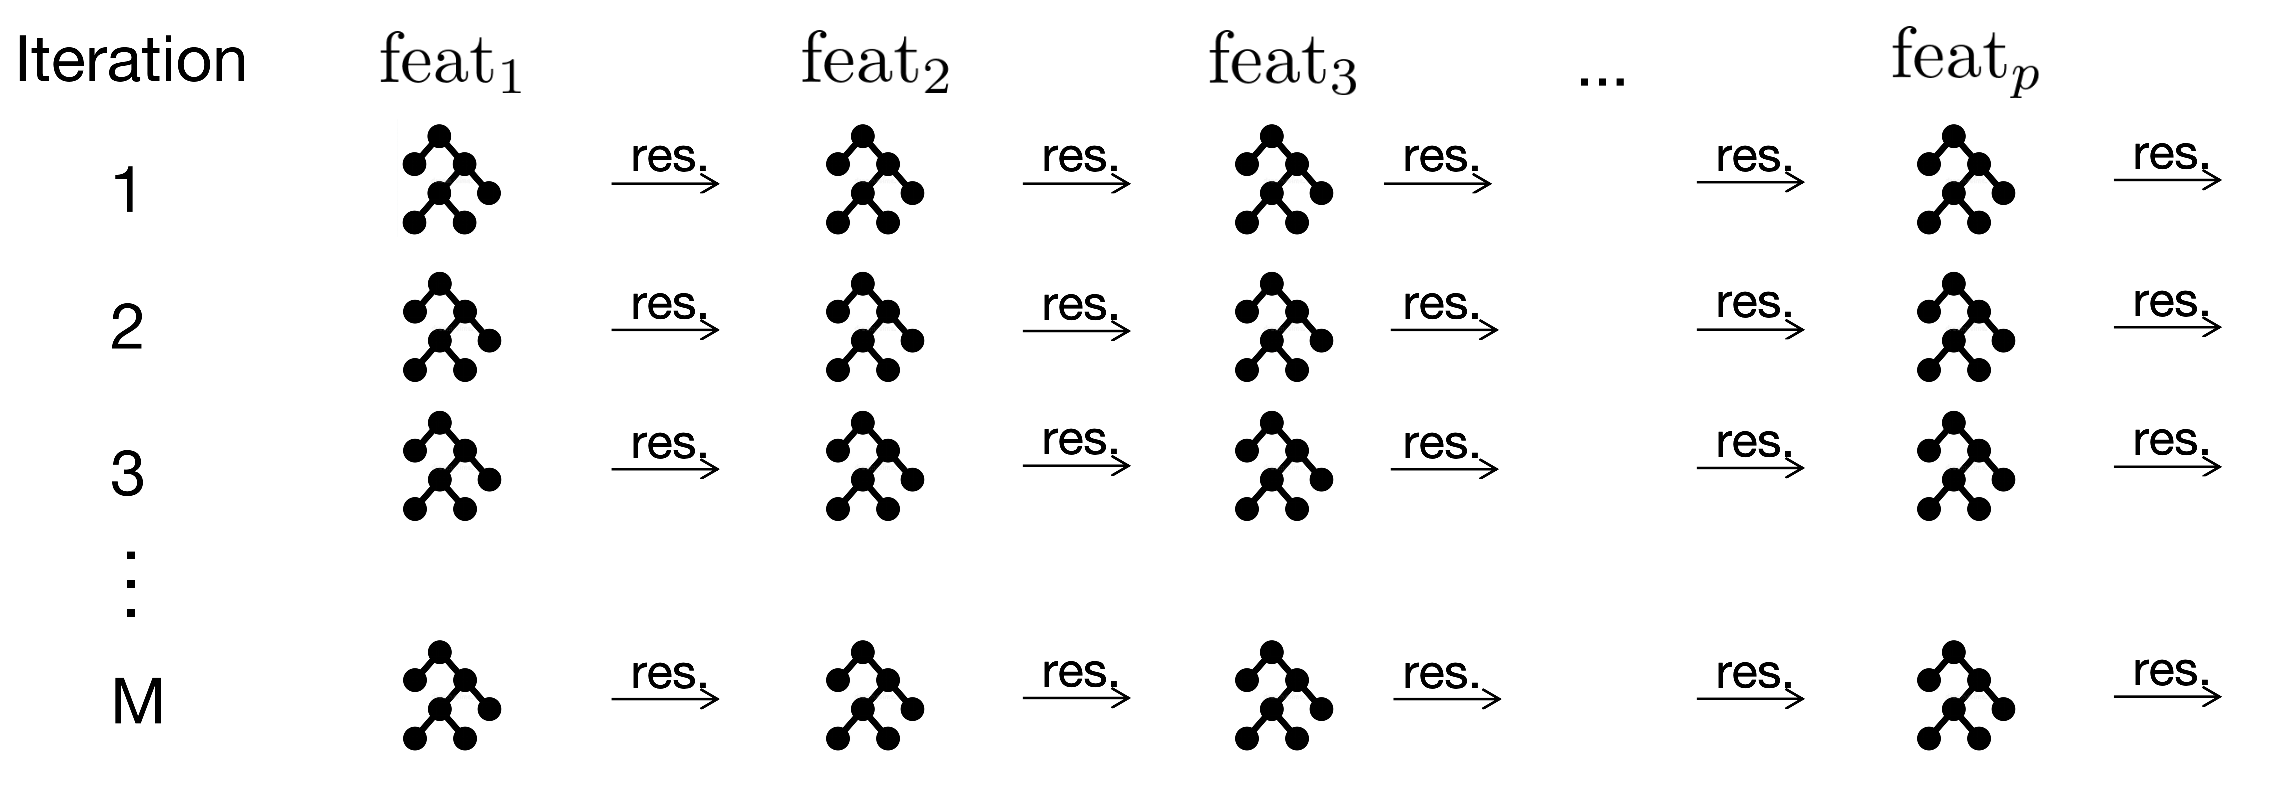
\includegraphics[width=\linewidth]{figure/EBM_Step3.png}
\end{figure}
\begin{itemize}
    \item Repeat feature-wise updates for $M$ boosting iterations (e.g., $M=10000$)
    \item In each boosting iteration:
    \begin{itemize}
        \item Cycle over all features $j=1,\dots,p$ individually %just one feature at a time 
        \item Update only one $f_j$ at a time using residuals from previous state
    \end{itemize}
    \item Use small learning rate $\eta$ to ensure smooth updates and order-invariance
\end{itemize}
\end{frame}














% \begin{frame}{Intelligible GAM - Algorithm Sketch - Part I}

% \begin{figure}
%     \centering
%     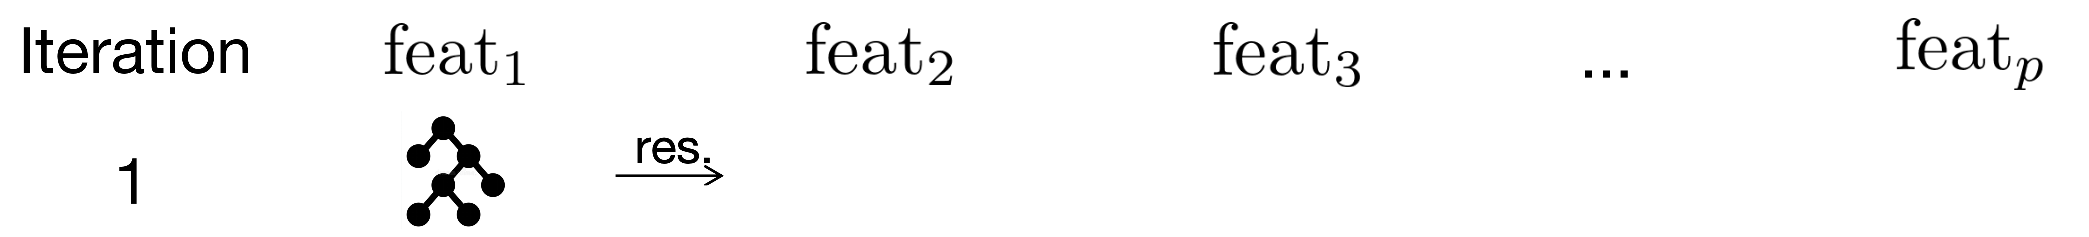
\includegraphics[width=1\linewidth]{figure/EBM_Step1.png}
%     \label{fig:Intelligible EBM_Step1}
% \end{figure}
% \begin{itemize}
%     \item Set all shape functions $f_j^{(0)}$ to zero, $j=1,\cdots,p$
%     \item Calculate the initial pseudo-residual (i.e. the negative gradient of the loss function w.r.t. the current model prediction), e.g.\\
%     1. for squared error loss: $\tilde{r}^{(0)}=-\frac{\partial L}{\partial \hat{y}}=y-\hat{y}^{(0)}=y-\sum_jf_j^{(0)}(x_{ij})$\\
%     2. for log loss: $\tilde{r}^{(0)}=-\frac{\partial L}{\partial \hat{y}}=y-\sigma(\hat{y}^{(0)})$ with $\sigma(\cdot)$ being the sigmoid function
%     \item Fit a shallow bagging tree with 2-4 leaves $S_1^{(1)}: x_{i1}\to \tilde{r}$ \textbf{only using the first feature} to predict the pseudo-residuals, with $\{x_{i1},\tilde{r}\}_1^N$ as training dataset
%     \item Update $f_1$: $f_1^{(1)}(x_{i1})=f_1^{(0)}+\eta\cdot S_1^{(1)}(x_{i1})$
%     \item Update $\hat{y}$: $\hat{y}^{(1)}=\sum_jf_j^{(1)}(x_{ij})$
%     \item Update the residual w.r.t. the original target, e.g. $\tilde{r}^{(1)}=y-\hat{y}^{(1)}$
%     \item Go to the second feature
% \end{itemize}
% \end{frame}

% \begin{frame}{Intelligible GAM - Algorithm Sketch - Part II}
% \begin{figure}
%     \centering
%     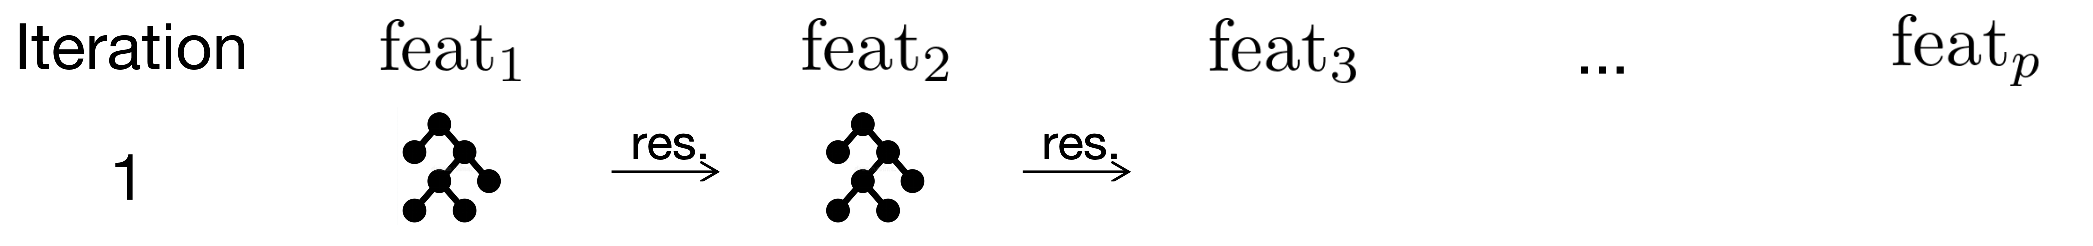
\includegraphics[width=1\linewidth]{figure/EBM_Step2.png}
%     \label{fig:Intelligible EBM_Step2}
% \end{figure}
% \begin{itemize}
%     \item Fit a shallow bagging tree $S_2^{(1)}$ \textbf{only using the second feature} to predict the updated residuals
%     \item Update $f_2$ with $f_2^{(1)}(x_{i2})=f_2^{(0)}+\eta\cdot S_2^{(1)}(x_{i2})$ and then update $\hat{y}^{(1)}$
%     \item Update the residual: this residual takes into account both what was learned on the first tree and second tree for the first two features
%     \item Go to $\text{feat}_3$
% \end{itemize}

% \end{frame}

% \begin{frame}{Intelligible GAM - Algorithm Sketch - Part III}
% \begin{figure}
%     \centering
%     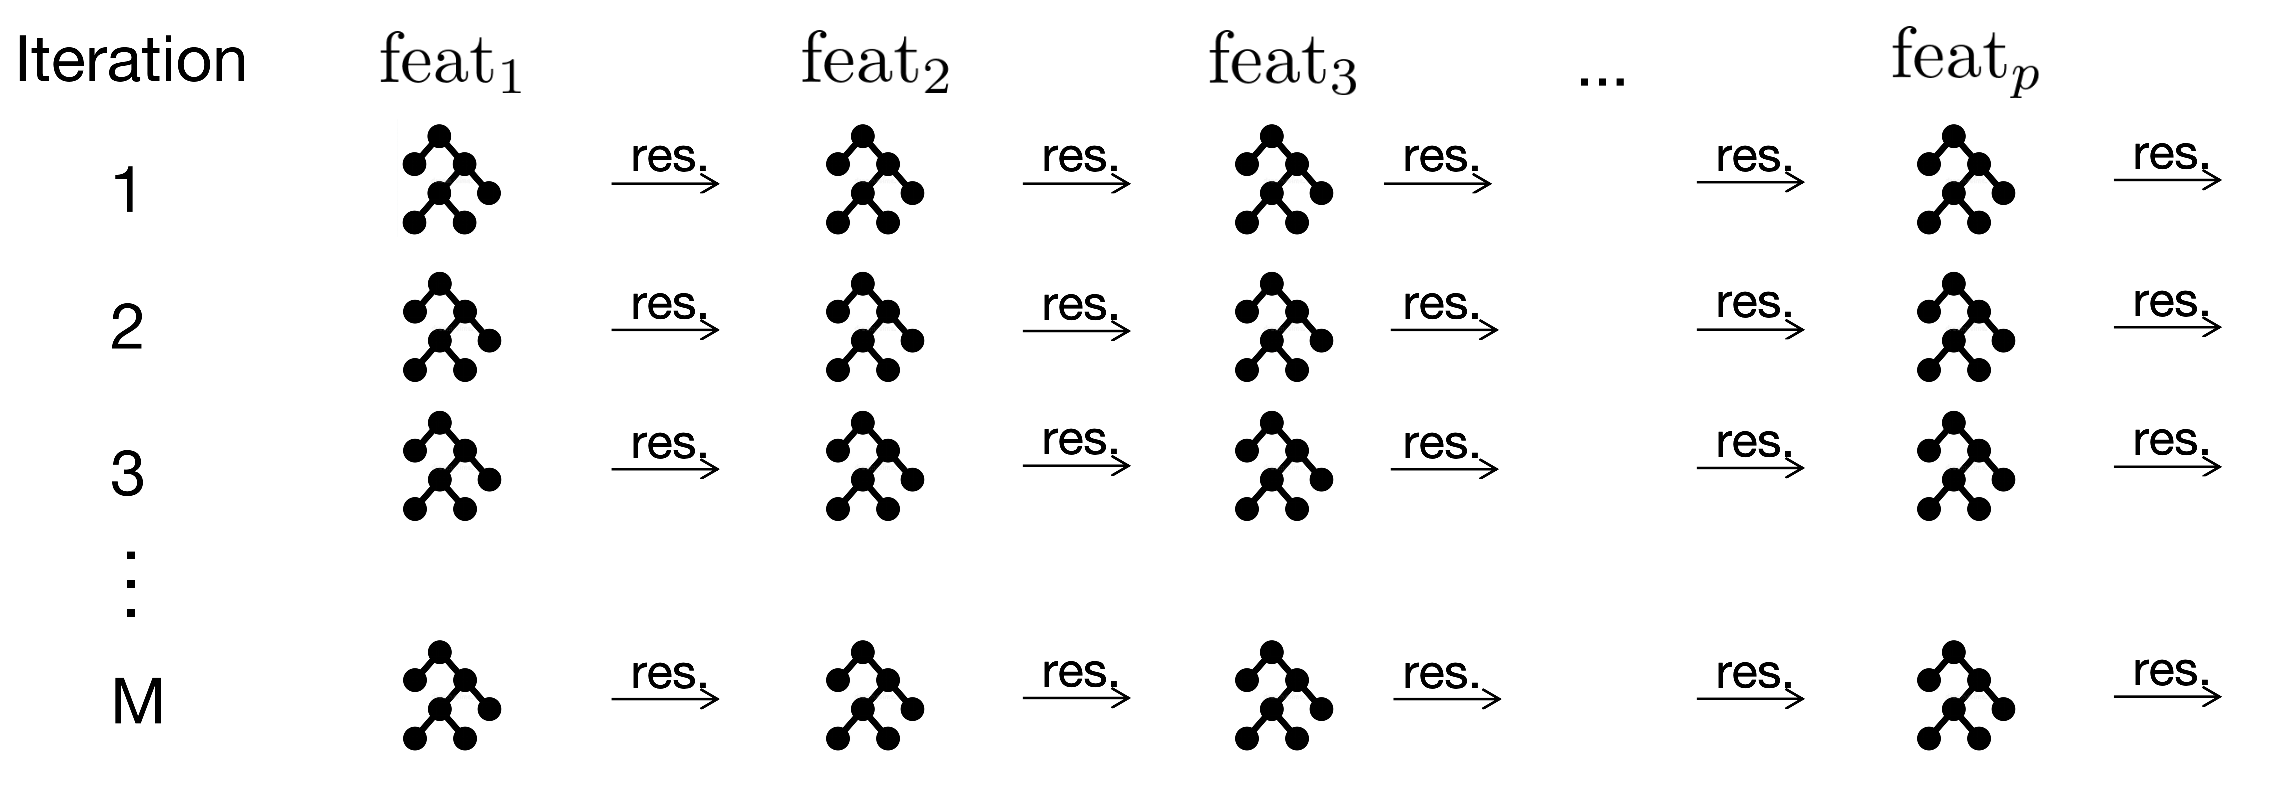
\includegraphics[width=1\linewidth]{figure/EBM_Step3.png}
%     \label{fig:Intelligible EBM_Step3}
% \end{figure}
% \begin{itemize}
%     \item Go through every feature and keep updating the residual
%     \item Grow a small tree on each feature but just one at a time in each iteration
%     \item Do $M$ iterations through these features until convergence (e.g. $M=10000$) \\
%     $\leadsto$ keep the learning rate $\eta$ so small that feature ordering does not matter
% \end{itemize}

% \end{frame}


\begin{frame}{EBM Stage I - Prediction and Interpretability}
\begin{itemize}
    \item Final model consists of $M$ shallow trees per feature:
    $$
    \text{EBM Model} = \sum_{j=1}^p \sum_{m=1}^M \eta \cdot S_j^{(m)}(x_j)
    $$
    \item For each feature $x_j$, combine its $M$ trees into a shape function:
    $$
    \hat{f}_j(x_j) = \sum_{m=1}^M \eta \cdot S_j^{(m)}(x_j)
    $$
    \item Plot $\hat{f}_j(x_j)$ vs. $x_j$ $\leadsto$ Shows univariate marginal effect of feature $j$
    \item One plot per feature $\leadsto$ Model is fully explainable via $p$ additive plots
\end{itemize}

\medskip

\begin{figure}
    \centering
    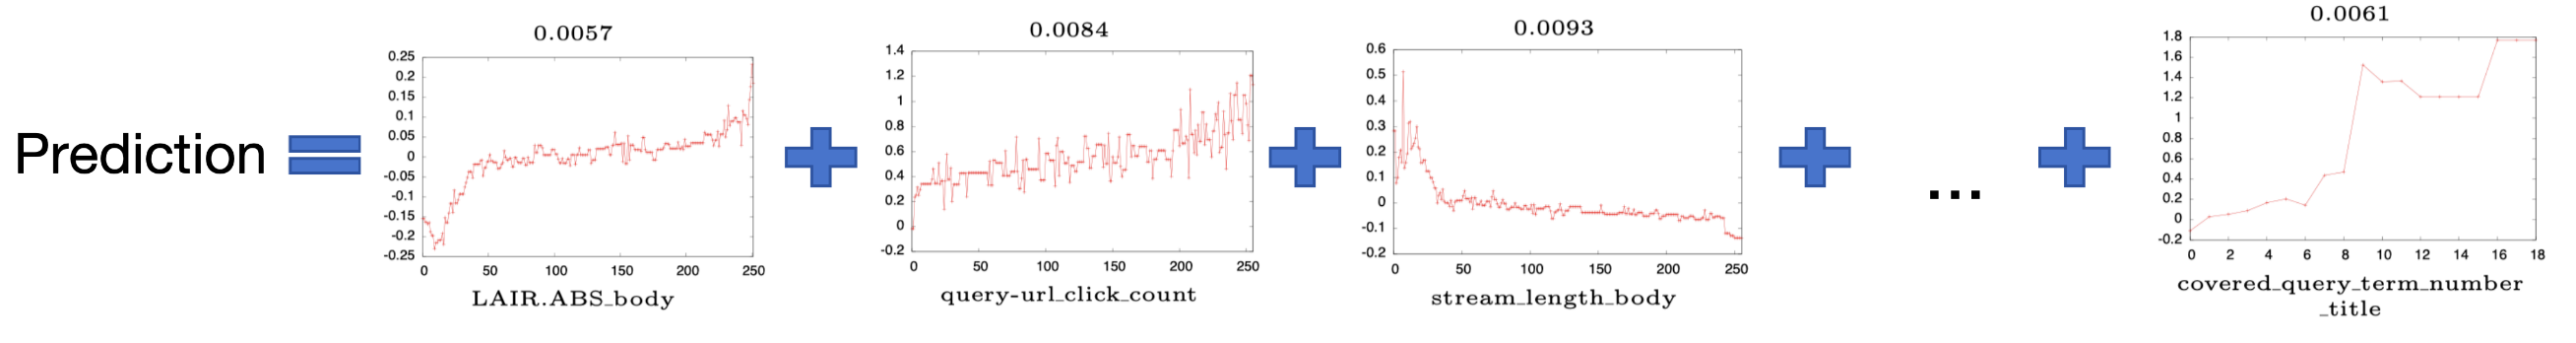
\includegraphics[width=\textwidth]{figure/ebm_prediction.png}
\end{figure}
\end{frame}


% \begin{frame}{Intelligible GAM - Prediction}
% \begin{itemize}
%     \item Output: $M$ trees which were only trained on $\text{feat}_1$ \\
%     \qquad\;\; + $M$ trees which were only trained on $\text{feat}_2$ \\
%     \qquad\;\; $\cdots$ \\
%     \qquad\;\; + $M$ trees which were only trained on $\text{feat}_p$
%     \item Summarize the weighted predictions of $M$ trees for each unique value of $\text{feat}_1$ $\hat{f}_1(x_1)=\sum_{m=1}^{M}\eta\cdot S_1^{(m)}(x_1)$, and plot $\hat{f}_1(x_1)$ vs. $x_1$ as a 2D graph
%     \item Generate a 2D graph for every feature in the same way
% \end{itemize}
% \quad $\leadsto$ Intelligible GAM: A series of 2D graphs as a perfect summary of predictions
% \begin{figure}
%     \centering
%     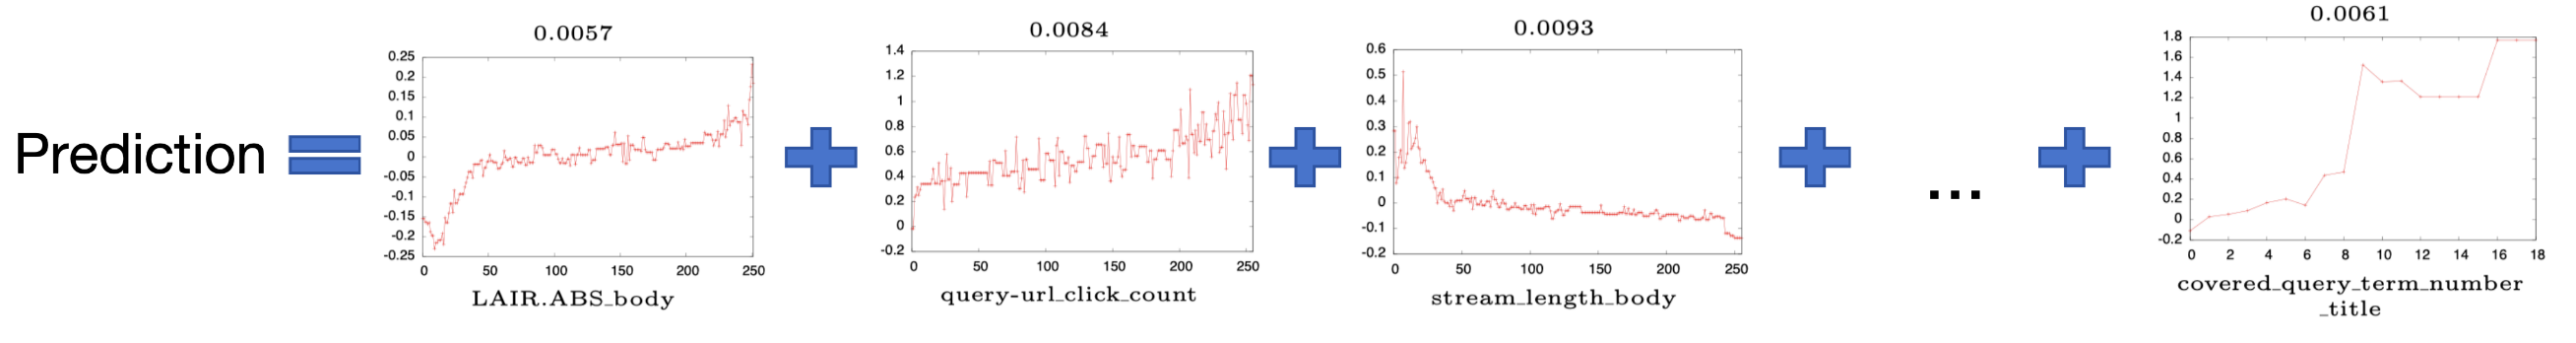
\includegraphics[width=\textwidth]{figure/ebm_prediction.png}
%     \label{fig:Intelligible ebm_prediction}
% \end{figure}
% \end{frame}

% \begin{frame}{Intelligible GAM - Novelty and Extension}
% \begin{itemize}
%     \item In each boosting step, use a bagging tree limited in size (2-4 leaves) \begin{itemize}
%         \item High accuracy, low variance, prevent overfitting
%         \item Provides discrete shape functions
%         \item Captures missing information in spline plots
%         \item High intelligibility
%     \end{itemize}
%     \item Not as accurate as unrestricted full complexity model
%     \item In the next step: \citebutton{Lou et al. 2013}{https://www.cs.cornell.edu/~yinlou/papers/lou-kdd13.pdf}
%     \begin{itemize}
%         \item Add pairwise feature interaction terms to the model
%         \item Replace the 2-4 regions of small tree
%         \item By a dynamic programming algorithm called FAST
%     \end{itemize}
% \end{itemize}
% \end{frame}

% \begin{frame}{Accurate GAM plus Pairwise Interactions}
% \textbf{Generalized Additive Models plus Interactions}: $$g(\E (y \mid \xv)) = \theta_0 + \sum f(x) + \sum f_{ij}(x,x_j)\quad for\quad i,j=1,\cdots,p,\quad i\neq j$$
% \begin{itemize}
%     \item $O(p^2)$: a large number of pairwise interactions if $p$ is big\\
%     $\leadsto$ Select only a small number of the most important interactions
%     \item Intuitively, significant reduction in RSS $\to$ Strong pair interaction
%     \item \textbf{FAST} algorithm does quick ranking without fully building every interaction function
% \end{itemize}
% \end{frame}


% \begin{frame}{GA2M - EBM \& Pairwise Interactions}
% \textbf{Generalized Additive Models plus Interactions (GA2M):}
% $$
% g\big(\mathbb{E}[y \mid \xv]\big) = \theta_0 + \sum_{j=1}^p f_j(x_j) + \sum_{i<j} f_{ij}(x_i, x_j)
% $$

% \begin{itemize}
%     \item \textbf{Extends EBM}: Adds selected bivariate functions $f_{ij}(x_i, x_j)$ to improve accuracy
%     \item \textbf{Interpretability preserved}: Each $f_{ij}$ is visualized as a 2D heatmap
%     \item Naively $O(p^2)$ possible pairs $\leadsto$ select only most relevant interactions
%     \item \textbf{FAST algorithm}: Ranks all feature pairs without exhaustively fitting them\\
%     $\leadsto$ Measures on how much a pair reduces residual sum of squares (RSS)
%     \item Top-ranked interactions added via a second-stage boosting step
% \end{itemize}
% \end{frame}

\begin{frame}{EBM Stage 2 - Include Pairwise Interactions}
\textbf{Generalized Additive Models plus Interactions (GA2M):}
$$
g\big(\mathbb{E}[y \mid \xv]\big) = \theta_0 + \sum_{j=1}^p f_j(x_j) + \sum_{i<j} f_{ij}(x_i, x_j)
$$

\begin{itemize}
    \item \textbf{Motivation}: EBM captures only univariate effects 
    $\leadsto$ misses interactions
    \item \textbf{Challenge}: $O(p^2)$ potential interactions
    $\leadsto$ infeasible %to include all pairs directly
    \item \textbf{Solution - FAST algorithm} \citebutton{Lou et al. 2013}{https://www.cs.cornell.edu/~yinlou/papers/lou-kdd13.pdf}:
    \begin{itemize}
        \item Efficiently estimates importance of all feature pairs
        \item Ranks pairs by reduction in residual sum of squares (RSS)
        \item Avoids full model fitting for each candidate
    \end{itemize}
    \item \textbf{Result}: Add only top-ranked interactions $f_{ij}$ via a second-stage boosting step\\
    $\leadsto$ Performed after the univariate EBM has been trained
    \item \textbf{Interpretability preserved}: Each $f_{ij}(x_i, x_j)$ visualized as a 2D heatmap
\end{itemize}
\end{frame}


\begin{frame}{FAST Feature Interaction Detection}
\begin{columns}[c, totalwidth=\textwidth]
\begin{column}{0.4\textwidth}
% \begin{figure}
%     \centering
%     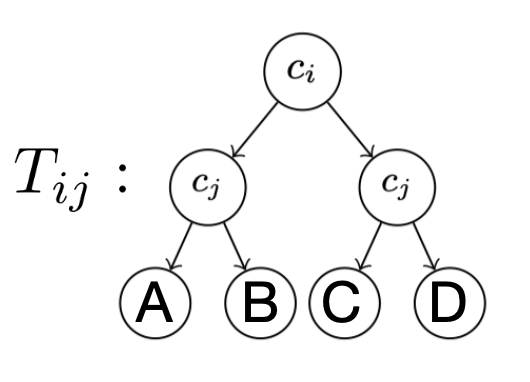
\includegraphics[width=0.8\linewidth]{figure/Tij.png}
% \end{figure}

\begin{figure}
\scalebox{0.85}{
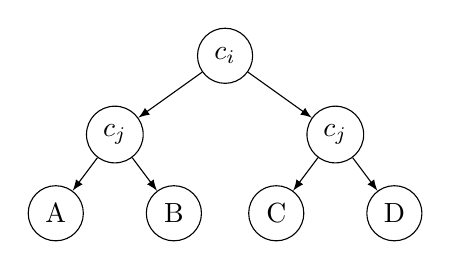
\begin{tikzpicture}[
  level 1/.style={sibling distance=28mm},
  level 2/.style={sibling distance=15mm},
  level distance=10mm,
  every node/.style = {circle, draw, minimum size=7mm},
  edge from parent/.style={draw,-latex}
]

\node (root) {$c_i$}
  child { node {$c_j$}
    child { node {A} }
    child { node {B} }
  }
  child { node {$c_j$}
    child { node {C} }
    child { node {D} }
  };

%\node[draw=none] at (-2.8,0.8) {$T_{ij}:$};

\end{tikzpicture}
}
\end{figure}

\end{column}
\hfill
\begin{column}{0.6\textwidth}
\begin{itemize}
    \item $T_{ij}$: Tree-like predictor with 4 leaf regions for a feature pair $(x_i, x_j)$
    \item Define axis-aligned cut points $(c_i, c_j)$ on the sorted values of $x_i$ and $x_j$
    \item Each split induces 4 regions: $A$, $B$, $C$, $D$
\end{itemize}
\end{column}
\end{columns}

\pause

\begin{columns}[c, totalwidth=\textwidth]
\begin{column}{0.4\textwidth}
\begin{figure}
\scalebox{0.9}{
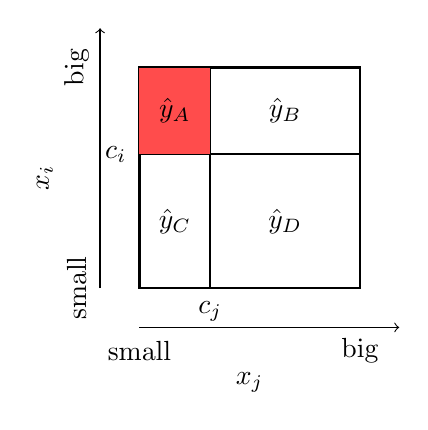
\begin{tikzpicture}[scale=1]

% Rectangle dimensions
\def\W{2.8}  % total width
\def\H{2.8}  % total height
\def\cx{0.9} % vertical cut
\def\cy{1.7} % horizontal cut

% Draw outer box and cuts
\draw[thick] (0,0) rectangle (\W,\H);
\draw[thick] (\cx,0) -- (\cx,\H);
\draw[thick] (0,\cy) -- (\W,\cy);

% Fill region a
\fill[red!70] (0,\cy) rectangle (\cx,\H);

% Region labels
\node at (0.45,2.25) {$\hat{y}_A$};
\node at (1.85,2.25) {$\hat{y}_B$};
\node at (0.45,0.85) {$\hat{y}_C$};
\node at (1.85,0.85) {$\hat{y}_D$};

% Axes
% x_j axis
\draw[->] (0,-0.5) -- (\W+0.5,-0.5);
\node at (0,-0.8) {small};
\node at (\W,-0.8) {big};
\node at (\W/2,-1.2) {$x_j$};

% x_i axis
\draw[->] (-0.5,0) -- (-0.5,\H+0.5);
\node[rotate=90] at (-0.8,0) {small};
\node[rotate=90] at (-0.8,\H) {big};
\node[rotate=90] at (-1.2,\H/2) {$x_i$};

% Cut point labels
\node at (\cx,-0.3) {$c_j$};
\node at (-0.3,\cy) {$c_i$};

\end{tikzpicture}
}
\end{figure}
\end{column}
\hfill
\begin{column}{0.6\textwidth}
\begin{itemize}
    \item Compute mean target in each region:
    $$
    \hat{y}_r = \frac{1}{|r|} \sum_{(\mathbf{x}, y) \in r} y, \quad r \in \{A, B, C, D\}
    $$
    \item Evaluate split quality via RSS:
    %$$\text{RSS}(c_i, c_j) = \sum_{i=1}^n (y^{(i)} - \hat{y}_r^{(i)})^2$$
$$\text{RSS}(c_i, c_j) = \sum_r \sum_{(\mathbf{x}, y) \in r} (y - \hat{y}_r)^2$$
    
    \item Goal: find cut $(c_i, c_j)$ minimizing RSS
\end{itemize}
\end{column}
\end{columns}
\end{frame}




\begin{frame}{FAST feature interaction detection}
For each pair of $(x_i,x_j)$ with $d_i$ and $d_j$ distinct values, calculate RSS for each possible $(c_i, c_j)$ and pick the best $T_{ij}$ with the lowest RSS ($\leadsto$ $N = d_i \cdot d_j$ different RSS values)

\begin{columns}[c, totalwidth=\textwidth]
    \begin{column}{0.45\textwidth}
\[
        \begin{array}{@{}l@{\quad}l@{\quad}l@{\quad}l@{\quad}l}
    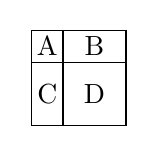
\begin{tikzpicture}[baseline=(current bounding box.center)]
        \draw (0,0) rectangle (1.2,1.2);
        \draw (0.4,0) -- (0.4,1.2); 
        \draw (0,0.8) -- (1.2,0.8); 
        \node at (0.2,0.4) {C};
        \node at (0.8,0.4) {D};
        \node at (0.2,1) {A};
        \node at (0.8,1) {B};
    \end{tikzpicture} & \text{$\Rightarrow$} & 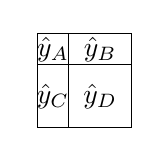
\begin{tikzpicture}[baseline=(current bounding box.center)]
        \draw (0,0) rectangle (1.2,1.2);
        \draw (0.4,0) -- (0.4,1.2); 
        \draw (0,0.8) -- (1.2,0.8); 
        \node at (0.2,0.4) {$\hat{y}_C$};
        \node at (0.8,0.4) {$\hat{y}_D$};
        \node at (0.2,1) {$\hat{y}_A$};
        \node at (0.8,1) {$\hat{y}_B$};
    \end{tikzpicture} & \text{$\Rightarrow$} & \text{$RSS_1$}\\[0.7cm] 
    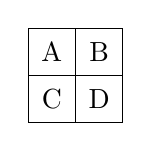
\begin{tikzpicture}[baseline=(current bounding box.center)]
        \draw (0,0) rectangle (1.2,1.2);
        \draw (0.6,0) -- (0.6,1.2); 
        \draw (0,0.6) -- (1.2,0.6); 
        \node at (0.3,0.3) {C};
        \node at (0.9,0.3) {D};
        \node at (0.3,0.9) {A};
        \node at (0.9,0.9) {B};
    \end{tikzpicture} & \text{$\Rightarrow$} & 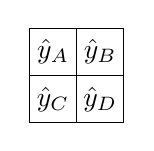
\begin{tikzpicture}[baseline=(current bounding box.center)]
        \draw (0,0) rectangle (1.2,1.2);
        \draw (0.6,0) -- (0.6,1.2); 
        \draw (0,0.6) -- (1.2,0.6); 
        \node at (0.3,0.3) {$\hat{y}_C$};
        \node at (0.9,0.3) {$\hat{y}_D$};
        \node at (0.3,0.9) {$\hat{y}_A$};
        \node at (0.9,0.9) {$\hat{y}_B$};
    \end{tikzpicture} & \text{$\Rightarrow$} & \text{$RSS_2$}\\[0.7cm] 
    \makebox[1cm][c]{\vdots} & & \makebox[1cm][c]{\vdots} & & \makebox[1cm][c]{\vdots}\\[0.3cm]
    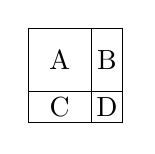
\begin{tikzpicture}[baseline=(current bounding box.center)]
        \draw (0,0) rectangle (1.2,1.2);
        \draw (0.8,0) -- (0.8,1.2); 
        \draw (0,0.4) -- (1.2,0.4); 
        \node at (0.4,0.2) {C};
        \node at (1,0.2) {D};
        \node at (0.4,0.8) {A};
        \node at (1,0.8) {B};
    \end{tikzpicture} & \text{$\Rightarrow$} & 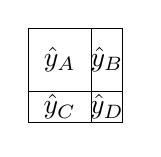
\begin{tikzpicture}[baseline=(current bounding box.center)]
        \draw (0,0) rectangle (1.2,1.2);
        \draw (0.8,0) -- (0.8,1.2); 
        \draw (0,0.4) -- (1.2,0.4); 
        \node at (0.4,0.2) {$\hat{y}_C$};
        \node at (1,0.2) {$\hat{y}_D$};
        \node at (0.4,0.8) {$\hat{y}_A$};
        \node at (1,0.8) {$\hat{y}_B$};
    \end{tikzpicture} & \text{$\Rightarrow$} & \text{$RSS_{N}$}\\ 
\end{array}
\]
    \end{column}
        \begin{column}{0.53\textwidth}
        For each candidate cut $(c_i, c_j)$:
  \begin{itemize}
    \item Divide 2D input space into 4 quadrants: A, B, C, D
    \item Compute average target $\hat{y}_r$ in each region $r \in \{A, B, C, D\}$
    \item Predict using a constant in each region
    \item Compute total RSS of this piecewise predictor
  \end{itemize}
Select the cut with minimal RSS - its value quantifies the interaction strength of $(x_i, x_j)$

    \end{column}
\end{columns}
% \medskip
% \textbf{Why is this fast?}\\
% Precompute cumulative sums (targets and counts) over sorted features\\
% $\leadsto$ Fast lookup of region totals for any cut $(c_i, c_j)$ without scanning data


%\text{\parbox[t]{6cm}{Select the lowest RSS and measure interaction strength of $(x_i, x_j)$ via risk reduction}}
\end{frame}


% \begin{frame}{RSS in FAST: Region-Based Derivation}
% \textbf{Objective:} Compute RSS for a 2D predictor $T_{ij}$ with four regions $r \in \{A, B, C, D\}$

% \medskip
% \textbf{Step 1: Expand squared residuals}
% \[
% \text{RSS}(c_i, c_j) = \sum_r \sum_{(x_k, y_k) \in r} (y_k - \hat{y}_r)^2
% = \sum_r \left( \sum_{(x_k, y_k) \in r} y_k^2 - 2 \hat{y}_r \sum_{(x_k, y_k) \in r} y_k + \hat{y}_r^2 \cdot |r| \right)
% \]

% \medskip
% \textbf{Step 2: Define region aggregates}
% \[
% S_r^{(1)} = \sum_{(x_k, y_k) \in r} y_k, \quad
% S_r^{(2)} = \sum_{(x_k, y_k) \in r} y_k^2, \quad
% N_r = |r|, \quad
% \hat{y}_r = \frac{S_r^{(1)}}{N_r}
% \]

% \medskip
% \textbf{Step 3: Substitute and simplify}
% \[
% \text{RSS}(c_i, c_j) = \sum_r \left( S_r^{(2)} - \frac{(S_r^{(1)})^2}{N_r} \right)
% \]

% \bigskip
% \textbf{Efficient computation:} All $S_r^{(1)}$, $S_r^{(2)}$, and $N_r$ can be precomputed and stored in lookup tables
% \end{frame}

\begin{frame}{RSS in FAST: Region-Based Derivation}

\textbf{Goal:} Efficiently compute RSS over $r \in \{A, B, C, D\}$ defined by cuts $(c_i, c_j)$

\textbf{Step 1: Expand squared residuals}
\[
\text{RSS}(c_i, c_j) = \sum_{r} \sum_{(x, y) \in r} (y - \hat{y}_r)^2
= \sum_{r} \left( \sum y^2 - 2 \hat{y}_r \sum y + \hat{y}_r^2 \cdot n_r \right)
\]

\textbf{Step 2: Define region-wise statistics}
\[
\mu_r = \frac{T_r}{n_r}, \quad
T_r = \sum_{(x, y) \in r} y, \quad
Q_r = \sum_{(x, y) \in r} y^2, \quad
n_r = |r|
\]

\textbf{Step 3: Substitute and simplify}
\[
\text{RSS}(c_i, c_j) = \sum_r \left( Q_r - \frac{T_r^2}{n_r} \right)
\]

\textbf{Why is this fast?}
\begin{itemize}
    \item Precompute cumulative sums of $y$, $y^2$, and counts
    \item Allows fast lookup of $T_r$, $Q_r$, and $n_r$ for any rectangle defined by $(c_i, c_j)$
\end{itemize}


\end{frame}



















% \begin{frame}{FAST feature interaction detection - PART I}

% \begin{columns}[T, totalwidth=\textwidth]
% \begin{column}{0.5\textwidth}
% \begin{figure}
%     \centering
%     \includegraphics[width=0.6\linewidth]
%     {figure/Tij.png}
%     \label{fig:tree-like predictor}
% \end{figure}
% \begin{figure}
%     \centering
%     \includegraphics[width=0.65\linewidth]
%     {figure/FAST1.png}
%     \label{fig:FAST1}
% \end{figure}
% \end{column}
% \hfill
% \centering
% \begin{column}{0.6\textwidth}
% \begin{itemize}
%     \item $T_{ij}$: A tree-like interaction predictor with 4 leaves for each pair of features
%     \item $c$, $c_j$: One cut (grid point) on the \textbf{sorted} values of feature $x$ and $x_j$, respectively
%     \item $A$, $B$, $C$, $D$: Notation for 4 leaf regions
%     \item \textbf{Idea}: Search for all possible $(c, c_j)$ and pick the best $T_{ij}$ with the lowest RSS
%     \item Prediction value on region r, $r\in\{A, B, C, D\}$:
%     $$\hat{y}_r=T_{ij}.r=\frac{1}{\vert r\vert}\sum_{(\mathbf{x},y)\in r}y=\frac{\text{Sum of targets in }r}{\text{Sum of counts in }r}$$
%     \item $\text{RSS}=\sum_{k=1}^N(y_k-T_{ij}(\mathbf{x}_k))^2$ \\
%     \qquad\;$=\sum_{k=1}^Ny_k^2-2\sum_r\left(\hat{y}_r\cdot\sum_{(\mathbf{x},y)\in r}y\right)$\\
%     \qquad\;\;\;\;$+\sum_r\hat{y}_r^2\cdot\vert r\vert$
% \end{itemize}
% \end{column}
% \end{columns}

% \end{frame}

% \begin{frame}{FAST feature interaction detection - PART II}

% \begin{columns}[T, totalwidth=\textwidth]
% \begin{column}{0.5\textwidth}
% \begin{itemize}
% \item How to quickly get sum of targets and sum of counts for all possible cuts?\\
%     $\leadsto$ Use \textbf{marginal cumulative histograms} (CH)
% \end{itemize}
% \begin{figure}
%     \centering
%     \includegraphics[width=\linewidth]
%     {figure/FAST.png}
%     \\An illustration for computing sum of targets for each quadrant
%     \label{fig:FAST2}
% \end{figure}
% \end{column}
% \hfill
% \centering
% \begin{column}{0.6\textwidth}
% \begin{itemize}
%     \item For example:\\
%     $CH_j^t(c_j)$: cumulative sum of targets for data points with $x_j\leq c_j$;\\
%     $\overline{CH_j^t }(c_j)$: cumulative sum of targets for data points with $x_j>c_j$
%     \item Create \textbf{two lookup tables} to store values for every $(c, c_j)$, :\\
%     1. Compute the cumulative sum of targets in four regions, and store the values in the \textbf{table of targets} $L^t(c,c_j)=[a,b,c,d]$\\
%     2. Compute the cumulative sum of counts in four regions, and store the values in the \textbf{table of counts} $L^w(c,c_j)=[a,b,c,d]$
%     \item Given any $(c, c_j)$, values of $(b,c,d)$ can be easily derived with known $\color{red}a$\\
%     $\leadsto$Construct lookup tables using dynamic programming
% \end{itemize}
% \end{column}
% \end{columns}

% \end{frame}

% \begin{frame}{FAST feature interaction detection - PART III}

% \begin{itemize}
%     \item For $x$ with $d$ possible values and $x_j$ with $d_j$ possible values:\\
%     $\leadsto$ compute and store $dd_j$ records of $[a,b,c,d]$ in both table of targets and table of counts
%     \item For each pair of $(x,x_j)$, calculate RSS for each possible $(c, c_j)$ and pick the best $T_{ij}$ with the lowest RSS [Note: $\hat{y}_A$ can be simply calculated as $L^t(c,c_j).a/L^w(c,c_j).a$]
% \end{itemize}
% \[
% \text{\qquad$dd_j$ possible $(c, c_j)$}
% \left\{
% \begin{array}{@{}l@{\quad}l@{\quad}l@{\quad}l@{\quad}l}
%     \begin{tikzpicture}[baseline=(current bounding box.center)]
%         \draw (0,0) rectangle (1.2,1.2);
%         \draw (0.4,0) -- (0.4,1.2); 
%         \draw (0,0.8) -- (1.2,0.8); 
%         \node at (0.2,0.4) {c};
%         \node at (0.8,0.4) {d};
%         \node at (0.2,1) {a};
%         \node at (0.8,1) {b};
%     \end{tikzpicture} & \text{$\Rightarrow$} & \begin{tikzpicture}[baseline=(current bounding box.center)]
%         \draw (0,0) rectangle (1.2,1.2);
%         \draw (0.4,0) -- (0.4,1.2); 
%         \draw (0,0.8) -- (1.2,0.8); 
%         \node at (0.2,0.4) {$\hat{y}_C$};
%         \node at (0.8,0.4) {$\hat{y}_D$};
%         \node at (0.2,1) {$\hat{y}_A$};
%         \node at (0.8,1) {$\hat{y}_B$};
%     \end{tikzpicture} & \text{$\Rightarrow$} & \text{$RSS_1$}\\[0.7cm] 
%     \begin{tikzpicture}[baseline=(current bounding box.center)]
%         \draw (0,0) rectangle (1.2,1.2);
%         \draw (0.6,0) -- (0.6,1.2); 
%         \draw (0,0.6) -- (1.2,0.6); 
%         \node at (0.3,0.3) {c};
%         \node at (0.9,0.3) {d};
%         \node at (0.3,0.9) {a};
%         \node at (0.9,0.9) {b};
%     \end{tikzpicture} & \text{$\Rightarrow$} & \begin{tikzpicture}[baseline=(current bounding box.center)]
%         \draw (0,0) rectangle (1.2,1.2);
%         \draw (0.6,0) -- (0.6,1.2); 
%         \draw (0,0.6) -- (1.2,0.6); 
%         \node at (0.3,0.3) {$\hat{y}_C$};
%         \node at (0.9,0.3) {$\hat{y}_D$};
%         \node at (0.3,0.9) {$\hat{y}_A$};
%         \node at (0.9,0.9) {$\hat{y}_B$};
%     \end{tikzpicture} & \text{$\Rightarrow$} & \text{$RSS_2$}\\[0.7cm] 
%     \makebox[1cm][c]{\vdots} & & \makebox[1cm][c]{\vdots} & & \makebox[1cm][c]{\vdots}\\[0.3cm]
%     \begin{tikzpicture}[baseline=(current bounding box.center)]
%         \draw (0,0) rectangle (1.2,1.2);
%         \draw (0.8,0) -- (0.8,1.2); 
%         \draw (0,0.4) -- (1.2,0.4); 
%         \node at (0.4,0.2) {c};
%         \node at (1,0.2) {d};
%         \node at (0.4,0.8) {a};
%         \node at (1,0.8) {b};
%     \end{tikzpicture} & \text{$\Rightarrow$} & \begin{tikzpicture}[baseline=(current bounding box.center)]
%         \draw (0,0) rectangle (1.2,1.2);
%         \draw (0.8,0) -- (0.8,1.2); 
%         \draw (0,0.4) -- (1.2,0.4); 
%         \node at (0.4,0.2) {$\hat{y}_C$};
%         \node at (1,0.2) {$\hat{y}_D$};
%         \node at (0.4,0.8) {$\hat{y}_A$};
%         \node at (1,0.8) {$\hat{y}_B$};
%     \end{tikzpicture} & \text{$\Rightarrow$} & \text{$RSS_{dd_j}$}\\ 
% \end{array}
% \right\}
% \text{\parbox[t]{6cm}{select the lowest RSS and assign it as the weight for $(x, x_j)$ to measure the strength of interaction}}
% \]
% \end{frame}

% \begin{frame}{FAST feature interaction detection - PART IV}
% \begin{itemize}
%     \item Complexity analysis: \\
%     Computing cumulative histograms: $O(N)$ ($N$: number of observations)\\
%     Constructing matrices of sum values: $O(N+dd_j)$\\
%     $\leadsto$ Complexity per pair: $O(N+dd_j)$ 
%     \item Discretize continuous feature values in $b$ bins ($b\leq256$)\\
%     $\leadsto O(N+b^2)$ per pair\\
%     $\leadsto$ Choose optimal number of bins $b$ w.r.t. bias-variance trade-off
%     \item Quick ranking and select top K pairs
% \end{itemize}
% \end{frame}

% \begin{frame}{GA2M - Two-stage Construction}
% \begin{enumerate}
%     \item Fit main effects
%     \begin{itemize}
%         \item Fit model only using univariate terms
%         \item Fix the main effects model
%     \end{itemize}
%     \item Fit pairwise residual of main effects model to original targets
%     \begin{itemize}
%         \item Use FAST to sort through $O(p^2)$ pairs
%         \item User selects number $K$ of pairs to be added
%         \item Run boosting algorithm to fit $K$ pairs
%         \item Final model = $p$ mains + $K$ pairs
%     \end{itemize}
% \end{enumerate}
% \end{frame}

% \begin{frame}{Accurate GAM - 2. Stage Algorithm Sketch}
% \begin{figure}
%     \centering
%     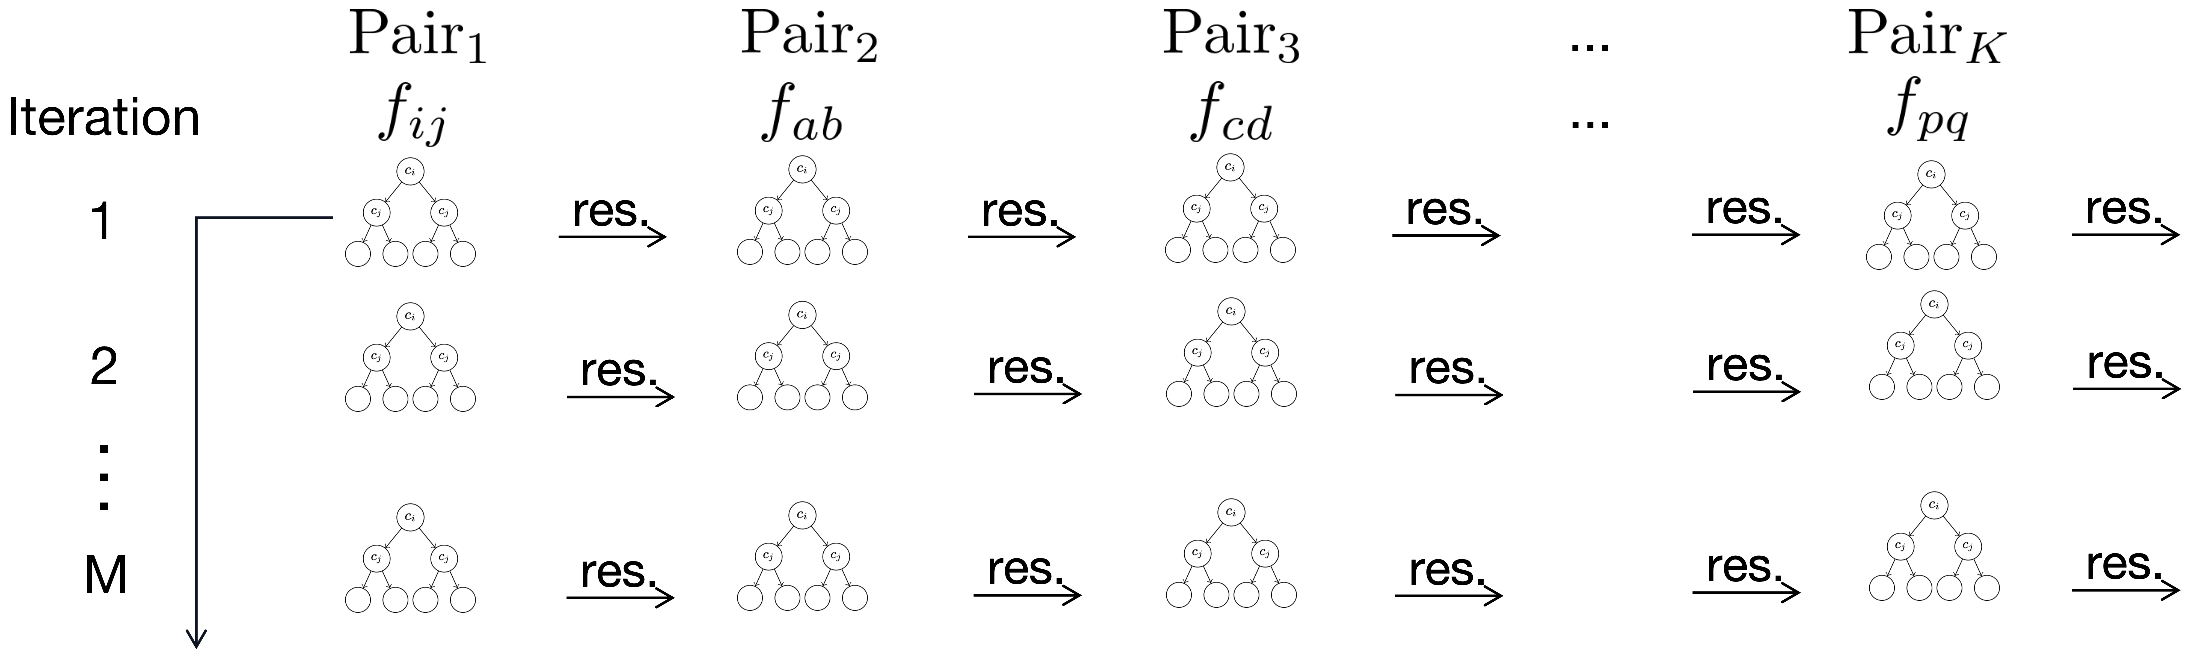
\includegraphics[width=1\linewidth]{figure/GA2M_Step1.png}
%     \label{fig:GA2M_Step1}
% \end{figure}
% \begin{columns}[T, totalwidth=\textwidth]
%     \begin{column}{0.4\textwidth} 
%         \begin{figure}
%             \vspace{-1.35cm} 
%             \hspace{-0.8cm} 
%             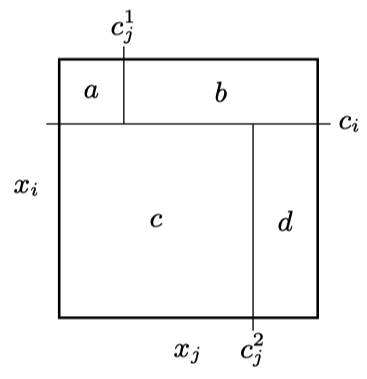
\includegraphics[width=0.8\linewidth]{figure/GA2M_Step0.png}
%             \label{fig:GA2M_predictor}
%         \end{figure}
%     \end{column}
%     \hfill
%     \begin{column}{0.7\textwidth}
%     \begin{itemize}
%       \setlength{\leftskip}{-0.7cm}
%       \vspace{-0.8cm}
%     \item Model each selected pairwise interaction $f_{ij}(x_i, x_j)$ using boosting over residuals
%     \item Replace shallow trees with a tree-like 2D predictor (similar to FAST) but use 3 cuts: 2 axis-aligned ($c_i$, $c_j$) and 1 additional refinement
%     \item Reuse precomputed lookup tables from FAST (sum of targets and counts per region)
%     \item Apply greedy search over cut positions to minimize RSS per boosting step
% \end{itemize}

%         % \begin{itemize}
%         %     \setlength{\leftskip}{-0.7cm}
%         %     \vspace{-0.8cm}
%         %     \item To model the pairwise interactions effectively and efficiently\\
%         %     $\leadsto$Replace the shallow tree ensembles used in Intelligible GAM with a tree-like predictor (similar to FAST)
%         %     \item 3 cuts instead of 2 cuts
%         %     \item Re-use the stored values in the lookup tables for sum of targets and sum of counts from FAST
%         %     \item Greedy search for the best combination of cuts (lowest RSS)
%         % \end{itemize}
%     \end{column}
% \end{columns}

% \end{frame}


\begin{frame}{EBM - Boosting Pairwise Interactions}
%\vspace{-0.2cm}
%\begin{figure}
%    \centering
    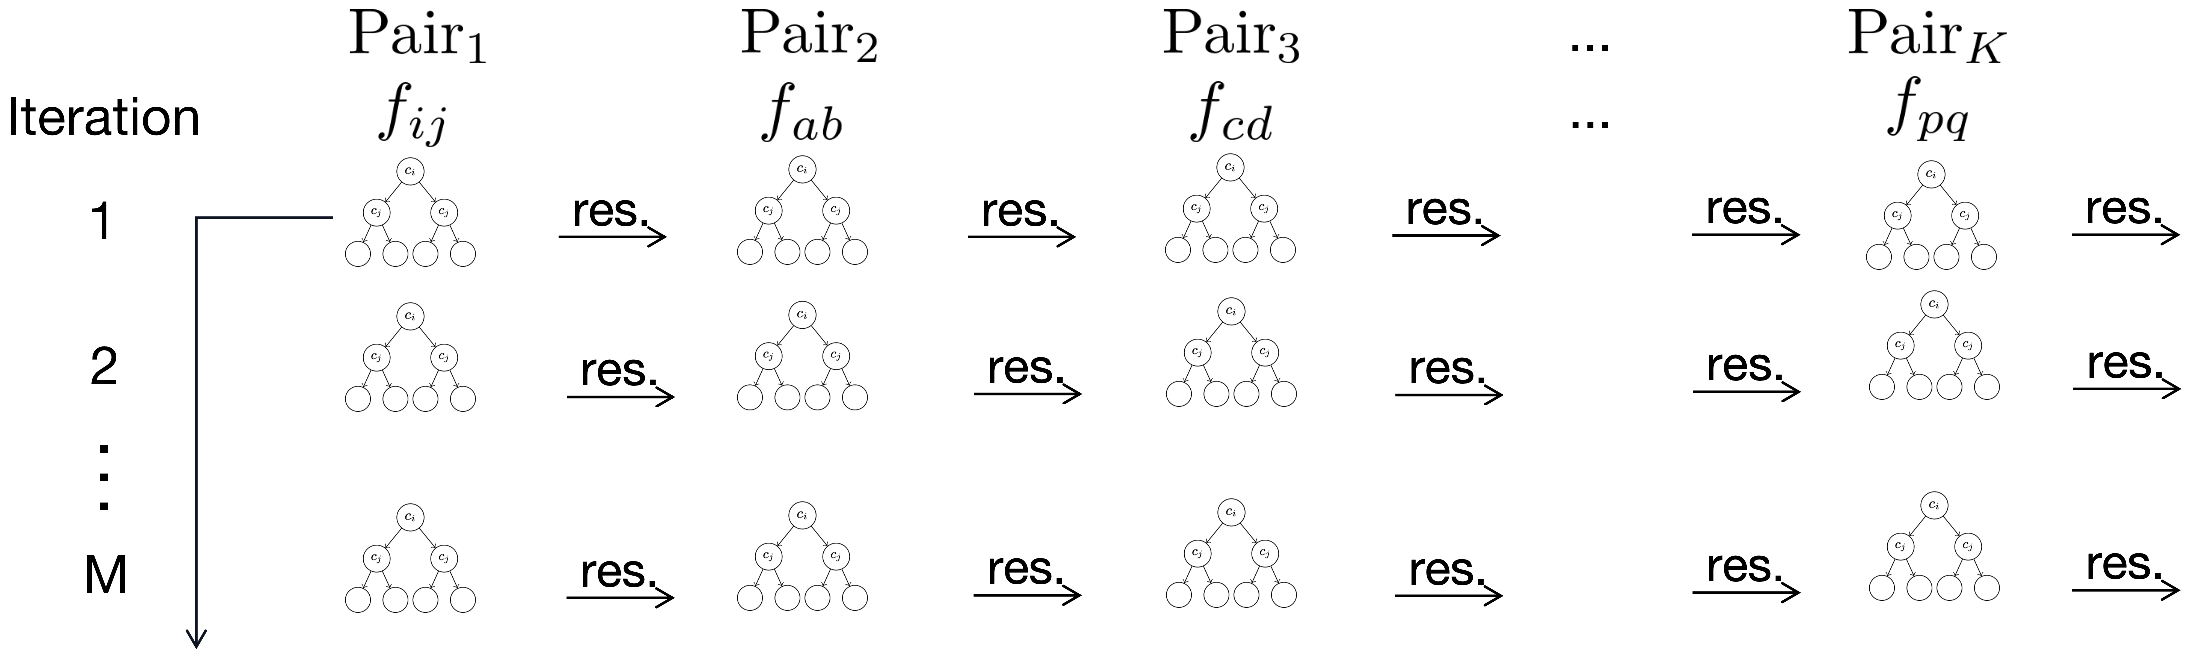
\includegraphics[width=\linewidth]{figure/GA2M_Step1.png}
%\end{figure}

\begin{columns}[c, totalwidth=\textwidth]
    \begin{column}{0.33\textwidth}
        % \vspace{-1.2cm}
        % \hspace{-0.6cm}
        %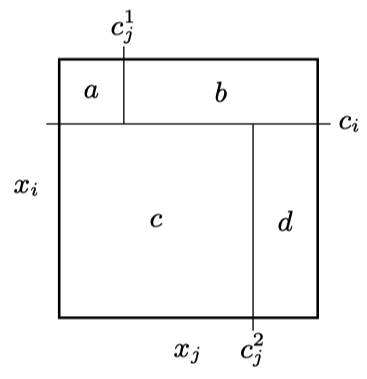
\includegraphics[width=\linewidth]{figure/GA2M_Step0.png}
\begin{center}
    \centering
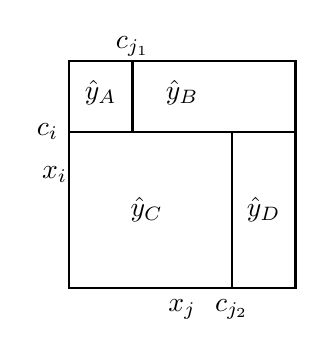
\begin{tikzpicture}[scale=0.9]

% Rectangle dimensions
\def\W{3.2}
\def\H{3.2}
\def\cxOne{0.9}
\def\cxTwo{2.3}
\def\cy{2.2}

% Outer box
\draw[thick] (0,0) rectangle (\W,\H);

% Internal cuts
\draw[thick] (\cxOne,\cy) -- (\cxOne,\H);
\draw[thick] (\cxTwo,0) -- (\cxTwo,\cy);
\draw[thick] (0,\cy) -- (\W,\cy);

% Region labels
\node at (0.45,2.75) {$\hat{y}_A$};
\node at (1.6,2.75) {$\hat{y}_B$};
\node at (1.1,1.1) {$\hat{y}_C$};
\node at (2.75,1.1) {$\hat{y}_D$};

% Axes and cut labels
\node at (-0.2,\H/2) {$x_i$};
\node at (\W/2,-0.3) {$x_j$};

\node at (-0.3,\cy) {$c_i$};
\node at (\cxOne,3.4) {$c_{j_1}$};
\node at (\cxTwo,-0.3) {$c_{j_2}$};

\end{tikzpicture}

\end{center}
    \end{column}
    
    \begin{column}{0.67\textwidth}
       % \vspace{-0.6cm}
        \begin{itemize}
            \item \textbf{Goal:} Fit each selected interaction $f_{ij}(x_i, x_j)$ on residuals from main effects
            \item Use tree-like predictor, inspired by FAST
            %\item \textbf{Cuts:} 
            \begin{itemize}
                \item Use two axis-aligned cuts $(c_i, c_j)$ 
                \item Plus one refinement cut to increase flexibility while keeping interpretability
            \end{itemize}
            \item Reuse region-wise sums from FAST lookup tables
            \item Greedy search for cut configuration minimizing RSS
        \end{itemize}
    \end{column}
\end{columns}
\end{frame}


% \begin{frame}{Accurate GAM - Prediction}
% \begin{itemize}
%     \item Output: $M$ predictors which were only trained on $\text{Pair}_1$ \\
%     \qquad\;\; + $M$ predictors which were only trained on $\text{Pair}_2$ \\
%     \qquad\;\; $\cdots$ \\
%     \qquad\;\; + $M$ predictors which were only trained on $\text{Pair}_K$
%     \item Summarize the weighted predictions of $M$ models in a 3D heatmap
%     \item The dimension of color represents the contribution of pairwise feature values to the prediction
%     \item Generate a 3D heatmap for each pair of features
% \end{itemize}

% \begin{figure}    
%     \includegraphics[width=0.4\linewidth]
%     {figure/3D Heatmap.png}
%     \label{fig:3D Heatmap}
% \end{figure}

% \end{frame}

% \begin{frame}{GA2M – Prediction with Pairwise Interactions}
% \begin{itemize}
%     \item Output: $M$ predictors for each of the $K$ selected pairwise interactions $f_{ij}(x_i, x_j)$
%     \item Each $f_{ij}$ is visualized as a 2D heatmap over feature pairs
%     \item Color encodes the contribution of feature value combinations to the final prediction
%     \item Summarize the ensemble of $M$ predictors per pair into a single interpretable surface
% \end{itemize}

% \vspace{0.3cm}
% \centering
% 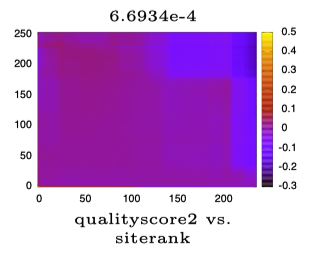
\includegraphics[width=0.42\linewidth]{figure/3D Heatmap.png}
% \end{frame}

\begin{frame}{EBM - Prediction with Pairwise Interactions}
\begin{itemize}
    \item Each selected pair $(x_i, x_j)$ is modeled by $M$ boosted predictors trained on their residual interaction
    \item These are aggregated into a single bivariate function $f_{ij}(x_i, x_j)$
    \item The function is visualized as a 2D heatmap: 
    \begin{itemize}
        \item Axes: feature values of $x_i$ and $x_j$
        \item Color: contribution to the final prediction
    \end{itemize}
    \item One heatmap is generated per selected pairwise interaction
\end{itemize}

\vspace{0.3cm}
\centering
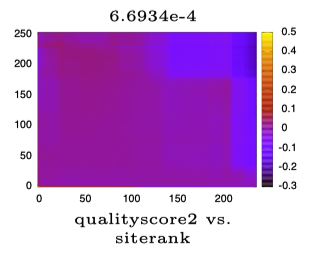
\includegraphics[width=0.42\linewidth]{figure/3D Heatmap.png}
\end{frame}


\begin{frame}{EBM - Final Model Structure}

\begin{itemize}
    \item \textbf{Main effects:} One shape function $f_j(x_j)$ per feature (visualized as 1D plots)
    \item \textbf{Pairwise interactions:} Selected functions $f_{ij}(x_i, x_j)$ added for top $K$ pairs (visualized as 2D heatmaps)
    \item \textbf{Prediction:} Additive sum of all univariate and selected bivariate contributions
\end{itemize}

\vspace{0.3cm}
\centering
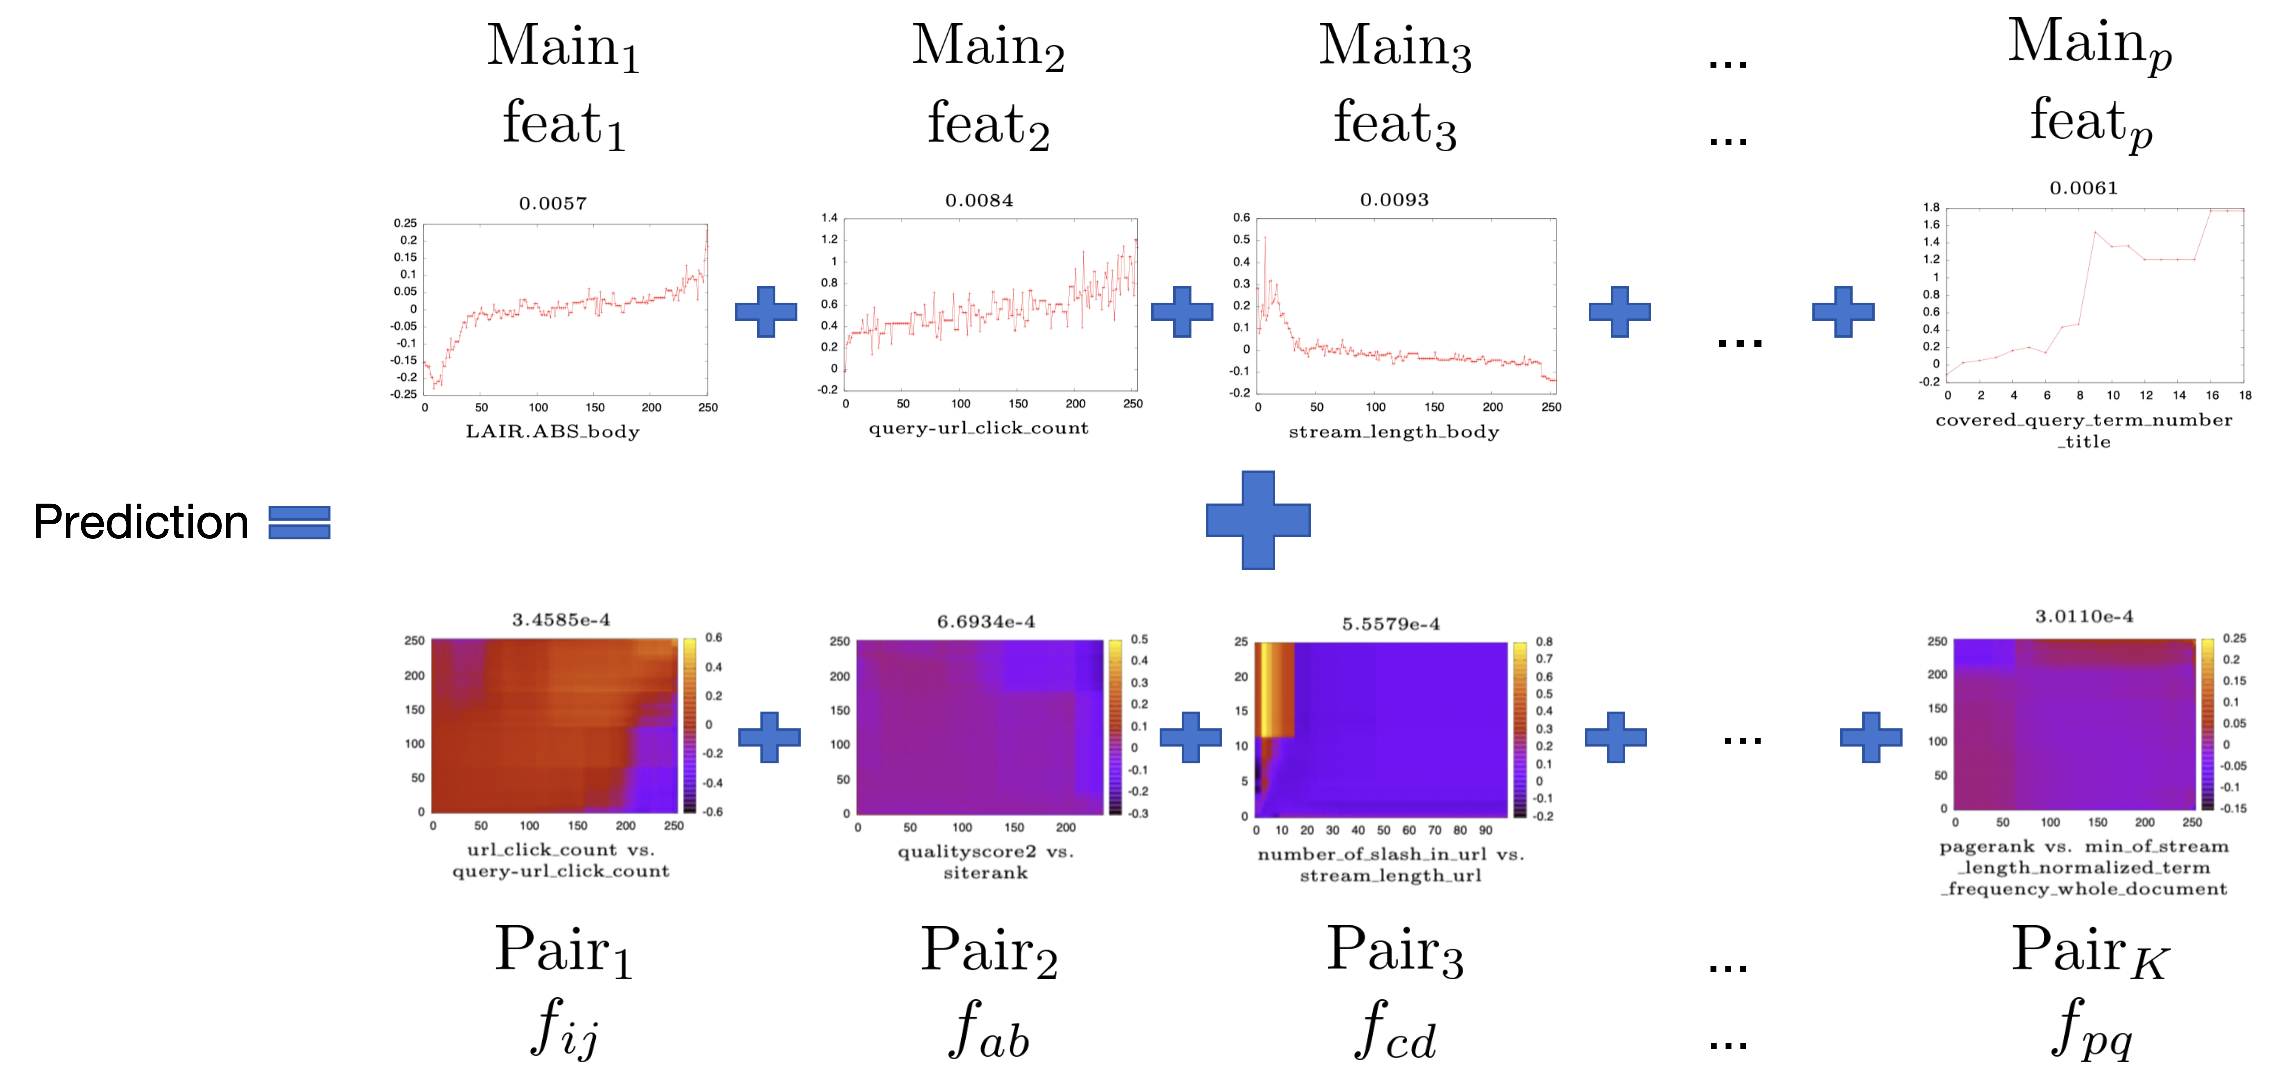
\includegraphics[width=\linewidth]{figure/final_ebm.png}

\end{frame}
\endlecture
\end{document}